\graphicspath{{Baro_vort/code/plot_snap/figs/}}

We start with perhaps the most simple model of geophysical turbulence, barotropic vorticity model. We can write the model in vorticity form \parencite[\S 4.2.1]{Vallis_17}:
\begin{align}
    &\frac{\DD}{\DD t}\left( \{\text{Ro}^{-1}\}f+\zeta \right) = 0,\\
    &\zeta = \nabla^2\psi,\\
    &u = -\frac{\pe\psi}{\pe y}, v = \frac{\pe\psi}{\pe x}.
\end{align}
where
\begin{align}
    \text{Ro} = \frac{U}{fL}.
\end{align}

If $f$ is constant, it is the 2D incompressible Euler equation. 

\section{Freely decaying simulation of 2D Euler}
We run freely decaying simulation with $f$ constant. We pick the initial energy containing scale of be around 1 and have a $15\times 15$ domain. We use $\nabla^8$ dissipation interpreted spectrally as $k^8+\ell^8$. 

Figure \ref{fig:2DEuler_zeta_t} shows the snap shots of vorticity and the streamfunction over the evolution of the simulation. We see a convincing inverse cascade and the formation of coherent vortices. Figure \ref{fig:2DEuler_energy} keep track of the kinetic energy and enstrophy. We see that, as expected, they experience a rapid initial decay. Afterwards, they are approximately conserved. Figure \ref{fig:2DEuler_spec} shows the evolution of the enstrophy spectra. The theoretical expectation is for them to have a $k^{-1}$ slope. We see that this is approximately true in early time. We also see that the hyper-dissipation is damping the small scale effectively.

\begin{figure}
    \centering
    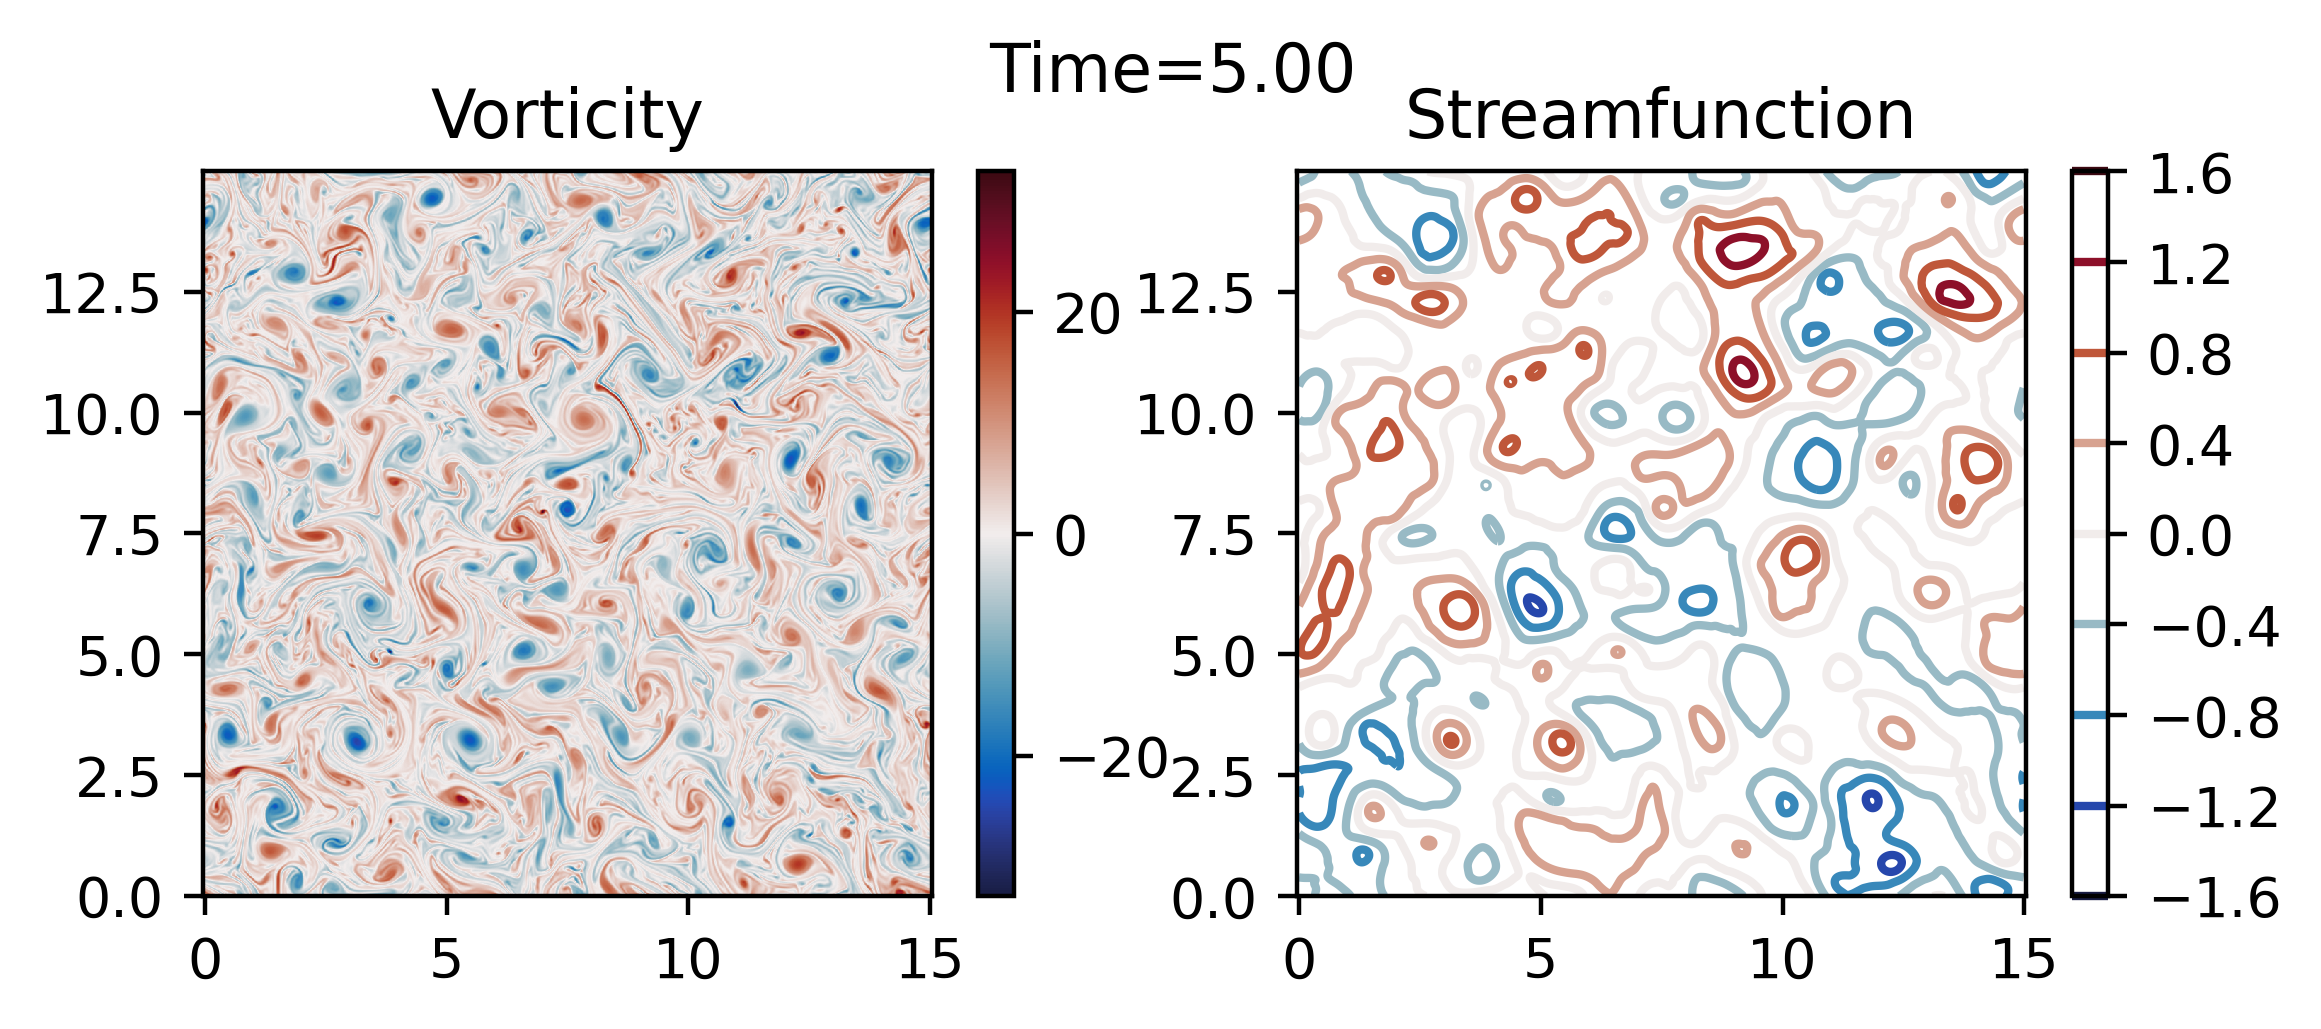
\includegraphics{2DEuler_zeta_t5d00}
    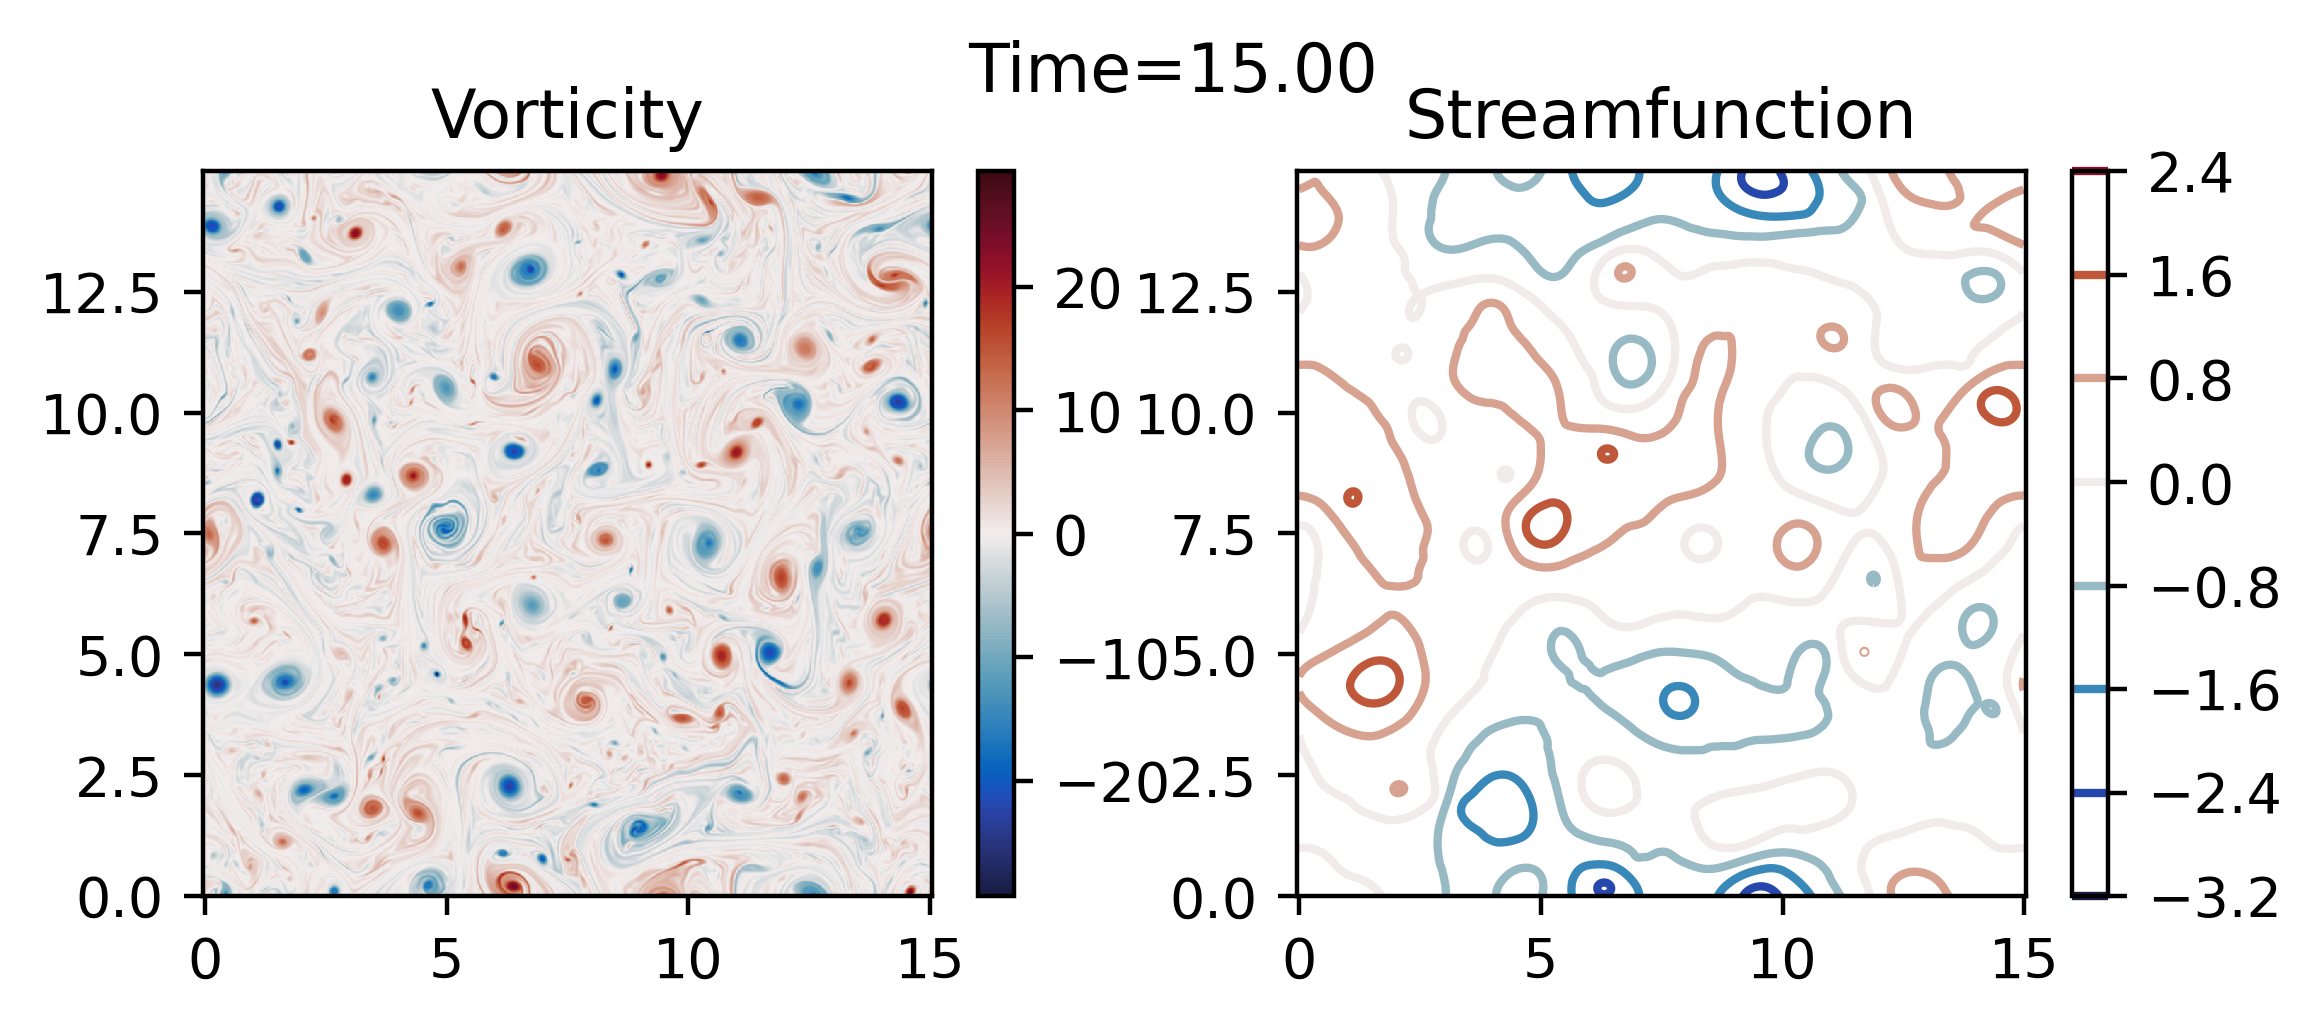
\includegraphics{2DEuler_zeta_t15d00}
    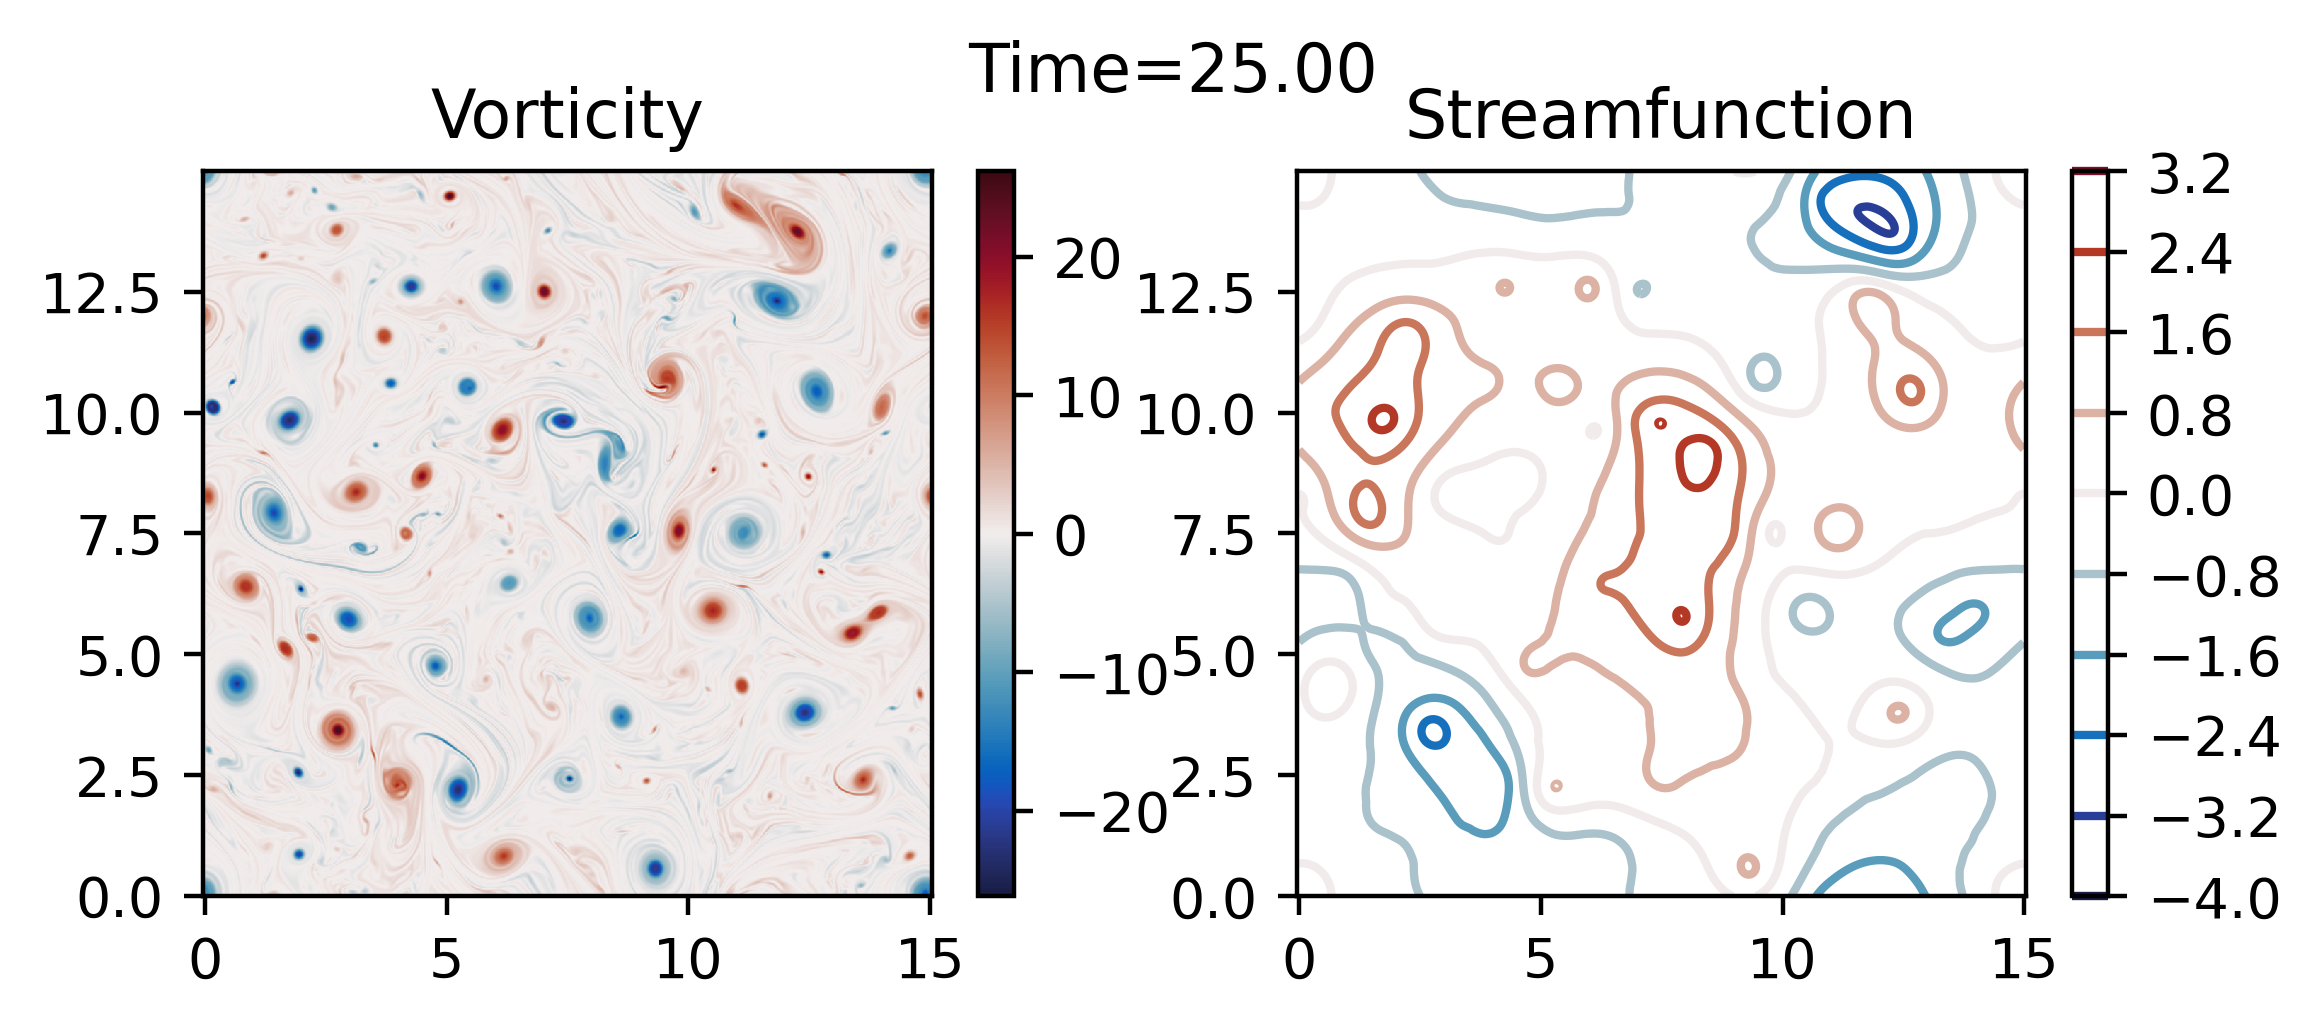
\includegraphics{2DEuler_zeta_t25d00}
    \caption{Snapshots of vorticity and streamfunction 2D Euler simulation overtime.}
    \label{fig:2DEuler_zeta_t}
\end{figure}

\begin{figure}
    \centering
    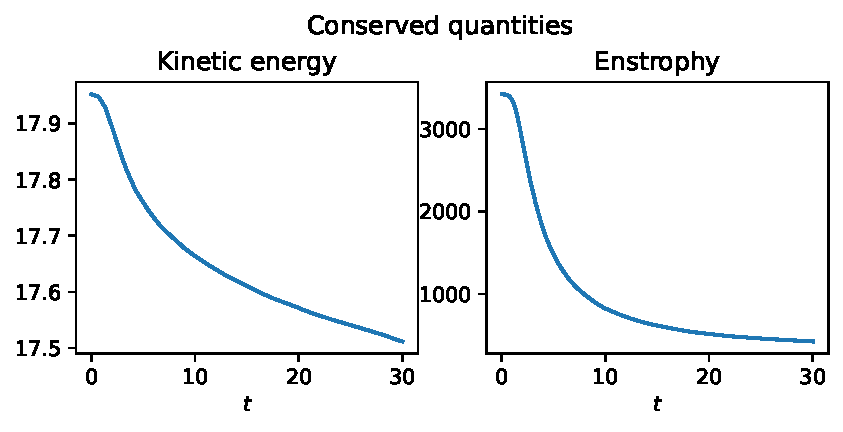
\includegraphics{2DEuler_energy}
    \caption{Time history of kinetic energy and enstrophy of 2D Euler simulation.}
    \label{fig:2DEuler_energy}
\end{figure}

\begin{figure}
    \centering
    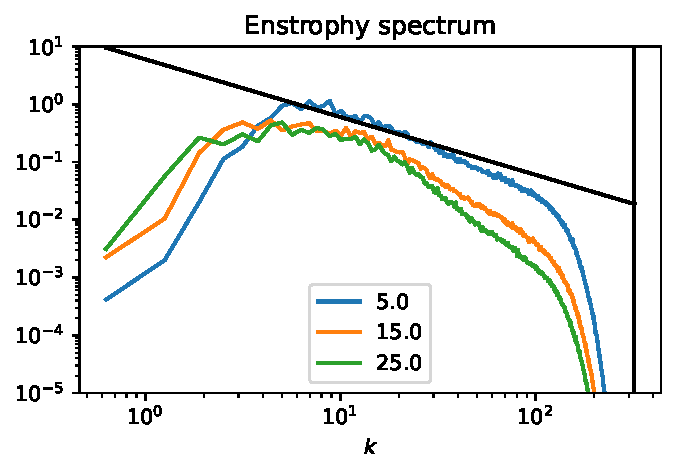
\includegraphics{2DEuler_spec}
    \caption{Time evolution of the enstrophy spectrum of 2D Euler simulation. Legends shows the time. The slanted black line is the $k^{-1}$ reference and the vertical black line is the maximally resolved wavenumber.}
    \label{fig:2DEuler_spec}
\end{figure}

% \section{Vortex crystal on a polar-cap}
% \cite[(2.2.10), p. 603]{Batchelor_53}

\section{Stochastically forced-dissipative simulation}

